\documentclass[11pt]{article}
\usepackage[a4paper, margin=2cm]{geometry}
\usepackage{graphicx}
\usepackage{amsmath}
\usepackage{array}
\usepackage{tabularx}
\usepackage{enumitem}

\pagestyle{empty}
\setlength{\parindent}{0pt}

\newcommand{\answerline}[1][3in]{\makebox[#1]{\hrulefill}}
\newcommand{\blankline}{\vspace{1cm}\hrule\vspace{0.2cm}}

\begin{document}
\begin{center}
	\textsc{This document contains Topic list and the Question paper}\\
	\textsc{*Each question might contain more than one topic }
\end{center}

\textbf{Topic List}
\begin{itemize}
    \item \textbf{Q1:} Motion or Kinematics, Forces or Dynamics
    \item \textbf{Q2:} Work Energy and Power
    \item \textbf{Q3:} Pressure, Kinetic Model of Matter
    \item \textbf{Q4:} General Wave Properties, Sound
    \item \textbf{Q5:} Electrical Quantities, Electric Circuits
    \item \textbf{Q6:} Electrical Quantities, Practical Electricity / Electrical Safety
    \item \textbf{Q7:} Electro Magnetism / Electromagnetic Induction
    \item \textbf{Q8:} Thermal Properties \& Temperature, The Nuclear Atom
    \item \textbf{Q9:} Forces or Dynamics, Earth \& Solar System
\end{itemize}
\newpage
\textbf{1} \quad A ball is dropped by the side of a vertical scale that is marked in centimetres.\\
A video recording of the fall shows the position of the ball on the scale every $0.10\text{ s}$.\\
The distance the ball falls is shown by the position on the scale.\\
Table 1.1 shows the results.

\begin{center}
Table 1.1\\[1ex]
\renewcommand{\arraystretch}{1.5}
\begin{tabular}{|l|c|c|c|c|c|c|}
\hline
time / s & 0 & 0.10 & 0.20 & 0.30 & 0.40 & 0.50 \\
\hline
distance / cm & 0 & 5 & 20 & 44 & 78 & 123 \\
\hline
\end{tabular}
\end{center}

\vspace{0.5cm}
\textbf{(a)} \textbf{(i)} \quad On Fig. 1.1, plot the distance-time graph for the ball. Draw a suitable line.
\hfill [2]

\begin{center}
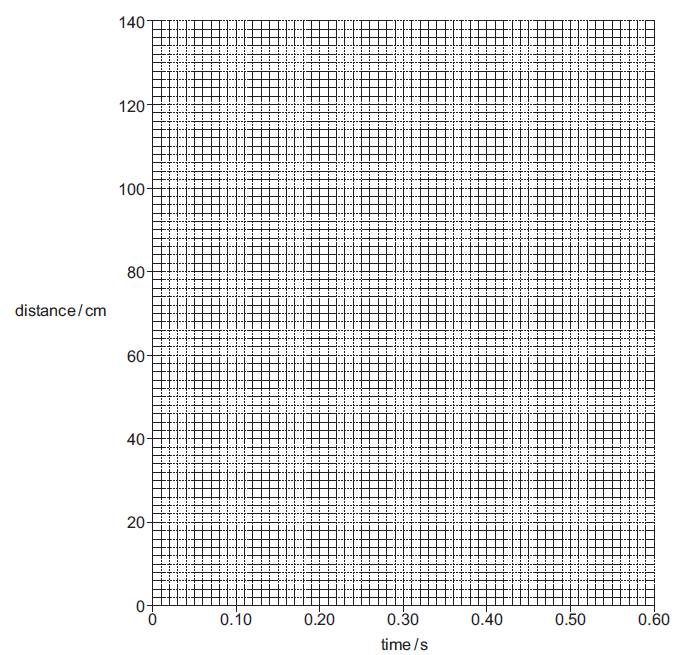
\includegraphics[\linewidth]{q1_fig1.1.png}
\end{center}

\newpage

\textbf{(ii)} \quad Calculate the average speed of the ball between time $t=0$ and time $t=0.40\text{ s}$.

\vspace{2cm}
\hfill speed = \answerline[2in] cm/s [2]

\vspace{0.5cm}
\textbf{(iii)} \quad Describe how to use the graph in Fig. 1.1 to determine the speed of the ball at time $t=0.40\text{ s}$.

\vspace{1cm}
\hrule
\vspace{0.8cm}
\hrule
\hfill [2]

\vspace{0.5cm}
\textbf{(b)} \quad As the ball falls, the acceleration of the ball decreases and eventually becomes zero before it reaches the ground.

\textbf{(i)} \quad Explain, in terms of the forces acting, why the acceleration decreases, and why it eventually becomes zero.

\vspace{1cm}
\hrule
\vspace{0.8cm}
\hrule
\vspace{0.8cm}
\hrule
\hfill [3]

\vspace{0.5cm}
\textbf{(ii)} \quad Describe the appearance of a distance-time graph when the acceleration of the ball is zero.

\vspace{1cm}
\hrule
\hfill [1]

\vspace{0.5cm}
\hfill [Total: 10]

\newpage

\textbf{2} \quad Fig. 2.1 shows a fork-lift truck used to lift a load.

\begin{center}
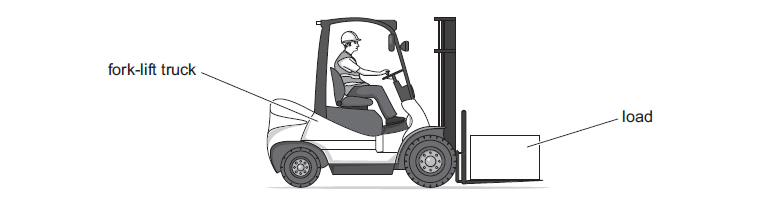
\includegraphics[width=0.10\linewidth]{q2_fig2.1.png}
\end{center}

When lifting the load, the electric motor on the fork-lift truck has a useful output power of 600 W.

\textbf{(a)} \quad Define `power'.

\vspace{1cm}
\hrule
\hfill [1]

\vspace{0.5cm}
\textbf{(b)} \quad The efficiency of the motor is 70\%.\\
Calculate the input power to the motor.

\vspace{2cm}
\hfill input power = \answerline[2in] W [2]

\vspace{0.5cm}
\textbf{(c)} \quad The fork-lift truck lifts a load with mass of 50 kg through a vertical distance of 2.3 m.

\textbf{(i)} \quad Calculate the work done in lifting the load.

\vspace{2cm}
\hfill work done = \answerline[2in] J [2]

\vspace{0.5cm}
\textbf{(ii)} \quad Calculate the time taken to lift the load.

\vspace{2cm}
\hfill time taken = \answerline[2in] s [2]

\vspace{0.5cm}
\textbf{(d)} \quad Describe how energy is transferred to thermal energy as the load is lifted by the fork-lift truck.

\vspace{1cm}
\hrule
\hfill [1]

\vspace{0.5cm}
\hfill [Total: 8]

\newpage

\textbf{3} \quad Fig. 3.1 shows a flat tyre on a car. The tyre needs to be inflated.

\begin{center}
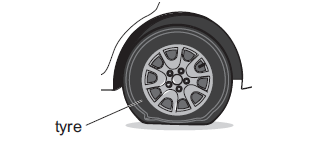
\includegraphics[width=0.6\linewidth]{q3_fig3.1.png}
\end{center}

\textbf{(a)} \quad The force exerted by the flat tyre on the road is 1350 N.\\
The area of the flat tyre in contact with the road is $0.0070\text{ m}^{2}$.

\textbf{(i)} \quad Calculate the pressure exerted by the flat tyre on the road.

\vspace{1cm}
\hfill pressure = \answerline[2in] Pa [2]

\vspace{0.5cm}
\textbf{(ii)} \quad Air is pumped into the tyre to inflate it. This increases the pressure inside. The force exerted by the tyre on the road does not change.\\
State how the area of the tyre in contact with the road changes.

\vspace{1cm}
\hrule
\hfill [1]

\vspace{0.5cm}
\textbf{(b)} \quad Inside the inflated tyre, a particle of air collides against the wall of the tyre.

\textbf{(i)} \quad Define `momentum'.

\vspace{1cm}
\hrule
\hfill [1]

\vspace{0.5cm}
\textbf{(ii)} \quad Using ideas about momentum, explain why there is a force on the wall of the tyre as the particle collides with it.

\vspace{1cm}
\hrule
\vspace{0.8cm}
\hrule
\vspace{0.8cm}
\hrule
\hfill [2]

\vspace{0.5cm}
\textbf{(c)} \quad As the car moves, the temperature of the air inside the tyre increases. The increase in temperature causes an increase in the pressure of the air.\\
Using ideas about particles, explain why the pressure increases.

\vspace{1cm}
\hrule
\vspace{0.8cm}
\hrule
\vspace{0.8cm}
\hrule
\hfill [2]

\vspace{0.5cm}
\hfill [Total: 8]
\newpage

\textbf{4} \quad A sound wave from a vibrating tuning fork is displayed on the oscilloscope shown in Fig. 4.1. The sound wave is detected using a microphone.

\begin{center}
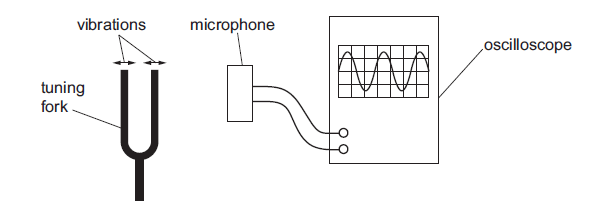
\includegraphics[width=0.9\linewidth]{q4_fig4.1.png}
\end{center}

\textbf{(a)} \quad Describe the motion of the air particles as the sound wave passes from the tuning fork to the microphone.

\vspace{1cm}
\hrule
\vspace{0.8cm}
\hrule
\vspace{0.8cm}
\hrule
\hfill [1]

\vspace{0.5cm}
\textbf{(b)} \quad Fig. 4.2 shows the trace seen on the oscilloscope when the tuning fork vibrates.

\begin{center}
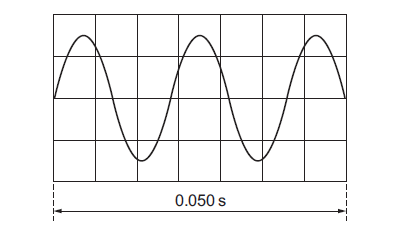
\includegraphics[width=0.6\linewidth]{q4_fig4.2.png}
\end{center}

The frequency of the sound is constant.

\textbf{(i)} \quad State what is meant by `frequency'.

\vspace{1cm}
\hrule
\vspace{0.8cm}
\hrule
\hfill [1]

\vspace{0.5cm}
\textbf{(ii)} \quad The trace shown on Fig. 4.2 is produced in 0.050 s.\\
Calculate the frequency of the sound wave.

\vspace{2cm}
\hfill frequency = \answerline[2in] Hz [2]

\newpage

\textbf{(iii)} \quad A student near the tuning fork observes the trace and listens to the sound. He notices that the amplitude of the trace decreases.\\
State how the sound heard by the student changes.

\vspace{1cm}
\hrule
\hfill [1]

\vspace{0.5cm}
\textbf{(iv)} \quad The tuning fork is replaced by a new tuning fork that produces a sound wave of half the frequency. The controls on the oscilloscope are not changed.\\
On Fig. 4.3, draw the trace obtained with the new tuning fork. The trace obtained with the original tuning fork is shown.

\begin{center}
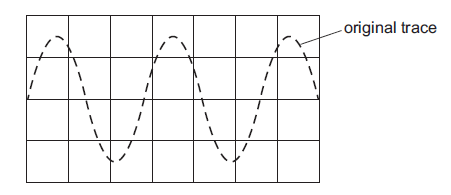
\includegraphics[width=0.8\linewidth]{q4_fig4.3.png}
\end{center}
\hfill [1]

\vspace{0.3cm}
\textbf{(c)} \quad Fig. 4.4 shows three adjacent wavefronts of the sound wave as the wavefronts move towards a gap in a wall created by an open door.\\
Another student, standing at P on the other side of the wall, hears the sound.

\begin{center}
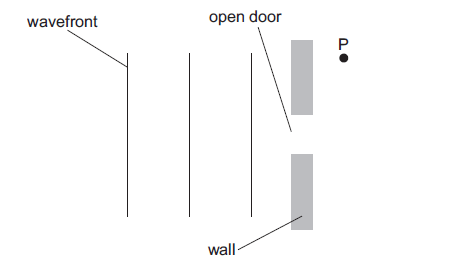
\includegraphics[width=0.7\linewidth]{q4_fig4.4.png}
\end{center}

\textbf{(i)} \quad On Fig. 4.4, draw the three wavefronts after they pass through the gap. \hfill [2]

\vspace{0.5cm}
\textbf{(ii)} \quad State the name of the process involved as the wavefronts pass through the gap and reach P.

\vspace{1cm}
\hrule
\hfill [1]

\vspace{0.5cm}
\hfill [Total: 10]

\newpage

\textbf{5} \quad A student sets up the circuit shown in Fig. 5.1 to measure the resistance of a length of wire. The circuit contains four identical cells.

\begin{center}
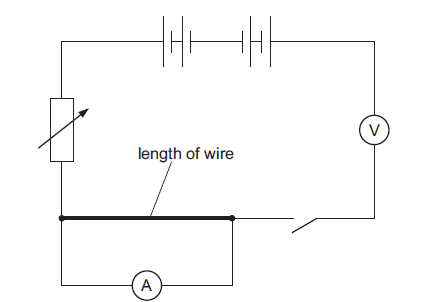
\includegraphics[width=0.7\linewidth]{q5_fig5.1.png}
\end{center}

The student finds that both meters read zero when the switch is closed. This is because the circuit shown in Fig. 5.1 is not suitable for the measurement.

\textbf{(a)} \quad Describe all the changes to the circuit in Fig. 5.1 that are needed so that the meters produce readings that can be used to calculate the resistance of the length of wire.

\vspace{1cm}
\hrule
\vspace{0.9cm}
\hrule
\vspace{0.9cm}
\hrule\vspace{0.9cm}
\hrule
\hfill [2]

\newpage

\textbf{(b)} \quad Fig. 5.2 shows the current-voltage graph for a 9.0 cm length of wire (line P) and for a different length of the same wire with the same cross-sectional area (line Q).

\begin{center}
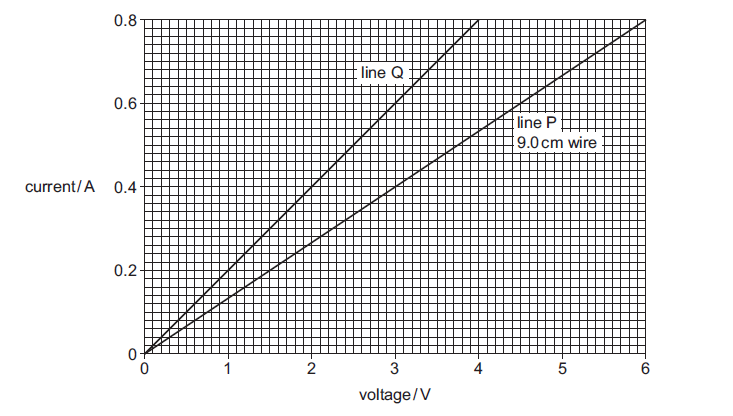
\includegraphics[width=0.99\linewidth]{q5_fig5.2.png}
\end{center}

\textbf{(i)} \quad Calculate the resistance of the 9.0 cm length of wire.

\vspace{2cm}
\hfill resistance = \answerline[2in] $\Omega$ [2]

\vspace{0.5cm}
\textbf{(ii)} \quad Explain whether line Q is obtained with a length of wire that is longer or shorter than 9.0 cm.

\vspace{1cm}
\hrule
\vspace{0.8cm}
\hrule
\hfill [1]

\vspace{0.5cm}
\textbf{(iii)} \quad Calculate the length of the wire used to obtain line Q.

\vspace{2cm}
\hfill length = \answerline[2in] cm [1]

\vspace{0.5cm}
\hfill [Total: 6]

\newpage

\textbf{6} \quad Fig. 6.1 shows part of a mains circuit that includes three lamps and a heater.

\begin{center}
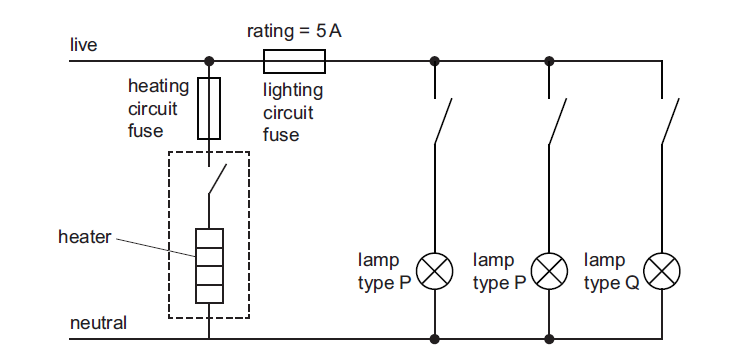
\includegraphics[width=0.99\linewidth]{q6_fig6.1.png}
\end{center}

\textbf{(a)} \quad The mains voltage is 230 V, and the power of the heater is 2000 W.\\
There is a 5 A fuse in the lighting circuit. Four fuses of different ratings are available for use in the heating circuit as shown in the list.\\
Underline the most suitable fuse value for the heating circuit fuse, and explain your choice. Your answer must include a calculation.

\vspace{0.5cm}
available fuses: \qquad 5 A \qquad 8 A \qquad 13 A \qquad 30 A

\vspace{0.9cm}
calculation

\vspace{1cm}
\hrule
\vspace{0.8cm}
\hrule

\vspace{0.5cm}
explanation

\vspace{1cm}
\hrule
\vspace{0.8cm}
\hrule
\vspace{0.8cm}
\hrule
\hfill [3]

\vspace{0.5cm}
\textbf{(b)} \quad Describe what happens to a fuse when the current is too large.

\vspace{1cm}
\hrule
\vspace{0.8cm}
\hrule
\hfill [1]

\newpage

\textbf{(c)} \quad Table 6.1 shows the current in lamps of type P and type Q when connected to the mains supply.

\begin{center}
Table 6.1\\[1ex]
\renewcommand{\arraystretch}{1.5}
\begin{tabular}{|l|c|}
\hline
lamp type & current / A \\
\hline
P & 0.26 \\
\hline
Q & 0.43 \\
\hline
\end{tabular}
\end{center}

\textbf{(i)} \quad Calculate the current in the lighting circuit fuse when all three lamps are switched on.

\vspace{2cm}
\hfill current = \answerline[2in] A [1]

\vspace{0.5cm}
\textbf{(ii)} \quad The rating for the lighting circuit fuse in Fig. 6.1 is 5 A.\\
The lamp of type Q is removed from the circuit.\\
Calculate the maximum number of additional lamps of type P that can now be connected in parallel to the lighting circuit.

\vspace{2cm}
\hfill number of additional lamps = \answerline[2in] [1]

\vspace{0.5cm}
\textbf{(d)} \quad In some houses the lighting circuit is protected by a trip switch (circuit breaker) instead of a fuse.\\
State two advantages of using a trip switch rather than a fuse.

\vspace{0.99cm}
1 \hrulefill
\vspace{0.99cm}
\hrule

\vspace{0.99cm}
2 \hrulefill \hfill [2]

\vspace{0.99cm}
\hrule
\vspace{0.99cm}
\hfill [Total: 8]

\newpage

\textbf{7} \quad Fig. 7.1 shows a simple d.c. motor. The poles at the ends of the magnets are not labelled.

\begin{center}
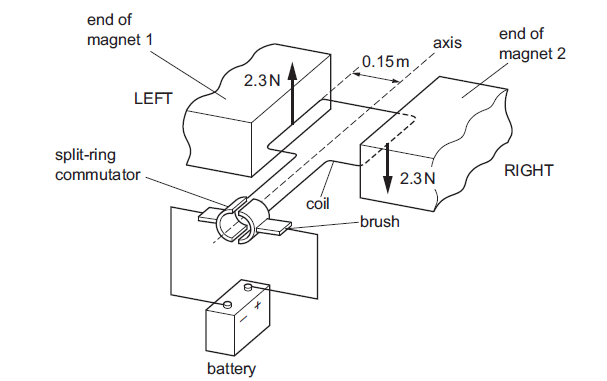
\includegraphics[width=0.9\linewidth]{q7_fig7.1.png}
\end{center}

\textbf{(a)} \quad State the purpose of the split-ring commutator and the brushes.

\vspace{0.5cm}
split-ring commutator \vspace{0.5cm} \hrule \vspace{0.8cm} \hrule

\vspace{0.5cm}
brushes \vspace{0.5cm} \hrule \vspace{0.8cm} \hrule \hfill [3]

\vspace{0.5cm}
\textbf{(b)} \quad There is an upward force shown on the left side of the coil.\\
There is a magnetic field in the space between the ends of the magnets.\\
State the direction of this magnetic field.\\
Explain how you determined this direction.

\vspace{0.5cm}
direction \vspace{0.5cm} \hrule \vspace{0.8cm} \hrule

\vspace{0.5cm}
explanation \vspace{0.5cm} \hrule \vspace{0.8cm} \hrule \hfill [3]

\newpage

\textbf{(c)} \quad State what happens to the rotation of the coil if the magnetic field and the current in the coil are both reversed at the same time.

\vspace{1cm}
\vspace{0.8cm}
\hrule
\vspace{0.8cm}
\hrule
\hrule
\hfill [1]

\vspace{0.5cm}
\textbf{(d)} \quad In Fig. 7.1, the coil is horizontal. The force upward on the left side and the force downward on the right side are each 2.3 N.\\
The distance between the sides of the coil and the axis is 0.15 m.

\textbf{(i)} \quad Calculate the total moment exerted on the coil by these forces.\\
Give the unit of your answer.

\vspace{2cm}
\hfill moment = \answerline[2in]

\vspace{1cm}
\hfill unit = \answerline[2in] \hfill [3]

\vspace{0.5cm}
\textbf{(ii)} \quad Explain why the turning effect becomes smaller as the coil becomes more vertical.

\vspace{0.8cm}
\hrule
\vspace{1cm}
\hrule
\hfill [1]
\vspace{0.8cm}
\hrule
\vspace{0.5cm}
\hfill [Total: 11]

\newpage

\textbf{8} \quad Fig. 8.1 is a diagram of a nuclear reactor.

\begin{center}
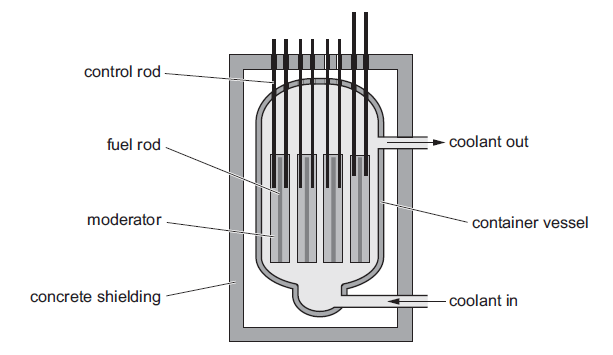
\includegraphics[width=0.99\linewidth]{q8_fig8.1.png}
\end{center}

Nuclear fission occurs within the fuel rods which become hotter as a result. The thermal energy is transferred to the coolant circulating around the rods.

\textbf{(a)} \quad In Table 8.1 state the purpose of each part of the reactor.

\begin{center}
Table 8.1\\[1ex]
\renewcommand{\arraystretch}{2}
\begin{tabular}{|p{4cm}|p{10cm}|}
\hline
\multicolumn{1}{|c|}{part} & \multicolumn{1}{c|}{purpose} \\
\hline
container vessel & to withstand high pressures and temperatures and make sure no coolant escapes \\
\hline
concrete shielding & \vspace{0.8cm}
\hrule \vspace{0.8cm}
\hrule \\
\hline
control rods & \vspace{0.8cm}
\hrule \vspace{0.8cm}
\hrule \\
\hline
moderator & \vspace{0.8cm}
\hrule \vspace{0.8cm}
\hrule \\
\hline
\end{tabular}
\end{center}
\hfill [3]

\newpage

\textbf{(b)} \quad Describe what causes the fission of a single nucleus of uranium-235 in the fuel rods, and describe what happens during the fission.

\vspace{1cm}
\hrule
\vspace{0.8cm}
\hrule
\vspace{0.8cm}
\hrule
\vspace{0.8cm}
\hrule
\hfill [3]

\vspace{0.5cm}
\textbf{(c)} \quad The specific heat capacity of the coolant is an important quantity in the design of the reactor.

\textbf{(i)} \quad State what is meant by `specific heat capacity'.

\vspace{1cm}
\hrule
\vspace{0.8cm}
\hrule
\vspace{0.8cm}
\hrule
\vspace{0.8cm}
\hrule
\hfill [2]

\vspace{0.5cm}
\textbf{(ii)} \quad Suggest and explain whether the coolant should have a large or a small specific heat capacity.

\vspace{1cm}
\hrule
\vspace{0.8cm}
\hrule
\vspace{0.8cm}
\hrule
\vspace{0.8cm}
\hrule
\hfill [1]

\vspace{0.5cm}
\hfill [Total: 9]

\newpage

\textbf{9} \quad Fig. 9.1 shows the path of a comet, the orbit of Earth and the orbit of Jupiter around the Sun.

\begin{center}
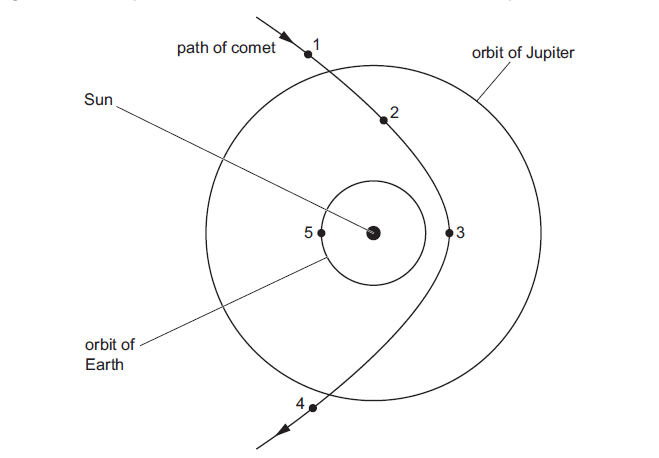
\includegraphics[width=0.99\linewidth]{q9_fig9.1.png}
\end{center}

The comet is at position 3 when Earth is at position 5.

\textbf{(a)} \quad On Fig. 9.1, draw the orbits of Mercury and Mars. Label each orbit. \hfill [2]

\vspace{0.5cm}
\textbf{(b)} \quad Explain why the comet at position 3 cannot be seen from Earth when Earth is at position 5.

\vspace{1cm}
\hrule
\vspace{0.8cm}
\hrule
\hfill [1]

\vspace{0.5cm}
\textbf{(c)} \quad A force causes the comet to orbit the Sun.

\textbf{(i)} \quad State the name of the force that acts on the comet.

\vspace{1cm}
\hrule
\vspace{0.8cm}
\hrule
\hfill [1]

\vspace{0.5cm}
\textbf{(ii)} \quad Four positions of the comet are shown in Fig. 9.1.\\
On Fig. 9.1, mark the direction of the force that acts on the comet at each of the four positions shown. \hfill [1]

\newpage

\textbf{(iii)} \quad Describe how the strength of the force that acts on the comet changes as the comet moves from position 1 through position 3 to position 4.\\
Explain your answer.

\vspace{0.5cm}
description \vspace{0.5cm} \hrule \vspace{0.8cm} \hrule

\vspace{0.5cm}
explanation \vspace{0.5cm} \hrule \vspace{0.8cm} \hrule \hfill [2]

\vspace{0.5cm}
\textbf{(d)} \quad Table 9.1 gives the orbital radius and the orbital speed of Earth and of Jupiter as each moves around the Sun.

\begin{center}
Table 9.1\\[1ex]
\renewcommand{\arraystretch}{1.5}
\begin{tabular}{|l|c|c|}
\hline
& orbital radius / km & orbital speed / km/s \\
\hline
Earth & $1.5 \times 10^{8}$ & 30 \\
\hline
Jupiter & $7.8 \times 10^{8}$ & 13 \\
\hline
\end{tabular}
\end{center}

Earth completes more orbits of the Sun than Jupiter in the same time.\\
Calculate the number of orbits that Earth makes around the Sun in the time that Jupiter makes one orbit.\\
Show your working.

\vspace{3cm}
\hfill number of orbits = \answerline[2in] [3]

\vspace{0.5cm}
\hfill [Total: 10]
\newpage

\end{document}